\documentclass[20pt]{beamer}

\usetheme{Berkeley}
\setbeamertemplate{caption}[numbered]
\everymath=\expandafter{\the\everymath\displaystyle}

\ifdefined\pdftexversion\else  % non-pdftex case.
	\usepackage{fontspec}
\fi
\makeatletter\@ifpackageloaded{underscore}{}{\usepackage[strings]{underscore}}\makeatother

\newcommand{\diff}[1]{\operatorname{d}#1}
\renewcommand{\vec}[1]{\boldsymbol{#1}}


\author{Henry Ding}
\date{\today}
\title{Lesson 7: Rotational Motion I} 


\begin{document}

\frame{\titlepage}

\section{Vector Cross Product}

\begin{frame}
	\frametitle{Cross Product}
	\begin{definition}
		The \textbf{vector cross product} ($\times$) is one way to multiply vectors in 3D. For vectors $\vec{u}, \vec{v}$, $\vec{u} \times \vec{v}$ gives a new vector perpendicular to both $\vec{u}$ and $\vec{v}$.
	\end{definition}
	\begin{figure}[ht]
		\centering
		\inkfig{0.3\textwidth}{crossproduct}
		%\caption{}
		\label{fig:crossproduct}
	\end{figure}
	\begin{theorem}
		If $\vec{u}$ and $\vec{v}$ are separated by $\theta$, magnitude of the cross product is
		\begin{align*}
		||\vec{u} \times \vec{v}|| = u v \sin \theta.
		\end{align*}
	\end{theorem}
	Note, if $\vec{u}$ and $\vec{v}$ are parallel, $\theta = 0$ so $\sin \theta = 0$theo.  Then, $\vec{u} \times \vec{v}$ has no magnitude.
\end{frame}

\begin{frame}
	\frametitle{Right Hand Rule for Cross Product}
	\begin{theorem}[Right Hand Rule]
		To find the direction of $\vec{u} \times \vec{v}$, use the right hand rule.
	\end{theorem}
	\begin{figure}[ht]
		\centering
		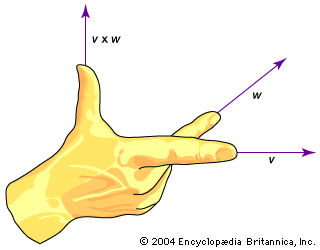
\includegraphics[width=0.6\textwidth]{righthandrulevector.png}
		%\caption{}
		\label{fig:righthandrulevector}
	\end{figure}
\end{frame}

\section{Rotation Motion}

\begin{frame}
	\frametitle{Rotational Motion}
	\begin{block}{What is Rotational Motion?}
		When objects rotate, they travel in circles about a \textbf{rotational axis}.
	\end{block}
	\begin{figure}[ht]
		\centering
		\inkfig{0.4\textwidth}{angularpos}
		%\caption{}
		\label{fig:angularpos}
	\end{figure}
	\begin{definition}
		The angular position $\theta$ of an object describes the orientation of an object relative to some reference.
		We can choose any pair of references and points on the object to define $\theta$.
	\end{definition}
\end{frame}

\begin{frame}
	\frametitle{Angular Velocity}
	\begin{definition}
		The average angular velocity $\vec{\omega}_\mathrm{avg}$ is a vector with magnitude
		\begin{align*}
			\omega_\mathrm{avg} = \frac{\Delta \theta}{\Delta t}.
		\end{align*}
		Just like regular instantaneous velocity $\vec{v}$ (sometimes called \textit{linear} velocity), we can define an instantaneous angular velocity $\vec{\omega}$.
		$\vec{\omega}$ points in the direction of the axis of rotation.
	\end{definition}
	\begin{figure}[ht]
		\centering
		\inkfig{0.46\textwidth}{angularvel}
		%\caption{}
		\label{fig:angularvel}
	\end{figure}
\end{frame}

\begin{frame}
	\frametitle{Right Hand Rule for Angular Velocity}
	\begin{theorem}[Right Hand Rule (Angular Velocity)]
		To determine the direction of $\vec{\omega}$, curl the fingers in your right hand around the direction of rotation. Then, $\vec{\omega}$ points in the direction of your thumb.
	\end{theorem}
	\begin{figure}[ht]
		\centering
		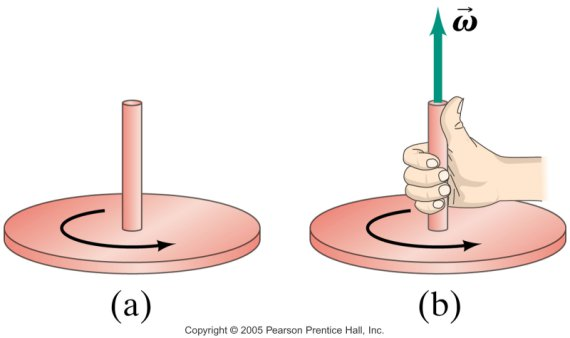
\includegraphics[width=0.6\textwidth]{righthandrule.jpeg}
		%\caption{}
		\label{fig:righthandrule}
	\end{figure}
	\begin{block}{Units for $\omega$}
		The units for angular velocity are $\SI{}{\radian/\second}$. However, radians are dimensionless, so sometimes the units are written as just $\SI{}{1/\second}$.
	\end{block}
\end{frame}

\begin{frame}
	\frametitle{Tangential Velocity from Angular Velocity}
	\begin{figure}[ht]
		\centering
		\inkfig{0.45\textwidth}{tangentialvel}
		%\caption{}
		\label{fig:tangentialvel}
	\end{figure}
	\begin{example}
		Consider a point at radius $r$ from the axis. Then, the arc length covered is
		\begin{align*}
			s = r \Delta \theta = (\omega \Delta t) r
		\end{align*}
		so the speed of the point is
		\begin{align*}
			v = \frac{s}{\Delta t} = \omega r.
		\end{align*}
	\end{example}
	\begin{theorem}
		A point at radius $r$ rotating with angular velocity $\omega$ has speed $r \omega$. The speed is in the tangential direction.
	\end{theorem}
\end{frame}

\begin{frame}
	\frametitle{Finding Velocity from the Right Hand Rule}
	\begin{theorem}
		A point at position $\vec{r}$ (measured relative to the axis) rotating with angular velocity $\vec{\omega}$ has velocity
		\begin{align*}
			\vec{v} = \vec{\omega} \times \vec{r}.
		\end{align*}
		$\vec{v}$ is often called \textbf{tangential velocity}, since it is tangent to the circle along which the point travels.
	\end{theorem}
	\begin{figure}[ht]
		\centering
		\inkfig{0.5\textwidth}{velcrossproduct}
		%\caption{}
		\label{fig:velcrossproduct}
	\end{figure}
	Note that $\vec{\omega}$ and $\vec{r}$ are perpendicular to each other. Then,
	\begin{align*}
		||\vec{v}|| = v = \omega r \sin (\pi / 2) = \omega r
	\end{align*}
	as expected.
\end{frame}

\begin{frame}
	\frametitle{Angular Acceleration}
	\begin{definition}
		Like linear acceleration, angular acceleration is
		\begin{align*}
			\vec{\alpha} = \frac{\Delta \vec{\omega}}{\Delta t}.
		\end{align*}
		$\vec{\alpha}$ is parallel to $\vec{\omega}$, so we can find the direction of both using the right hand rule.
	\end{definition}
	\begin{theorem}[Angular Kinematic Equations in One Dimension]
		When we have constant angular acceleration, the kinematic equations are in the same form
		\begin{align*}
			\omega_f                & = \omega_i + \alpha t                          \\
			\Delta \theta           & = \left(\frac{\omega_i + \omega_f}{2}\right) t \\
			\Delta \theta           & = \omega_i t + \frac{1}{2}\alpha t^2           \\
			\omega_f^2 - \omega_i^2 & = 2 \alpha \Delta \theta.
		\end{align*}
	\end{theorem}
\end{frame}

\begin{frame}
	\frametitle{Constant Angular Acceleration Examples}
	\begin{example}
		A CD disk undergoes constant angular acceleration from rest to rotating at $\SI{5}{\radian/\second}$ in $\SI{10}{\second}$. What is the disk's angular acceleration? Through what angle did the disk turn?
	\end{example}
\end{frame}

\section{Homework 7}

\begin{frame}
	\frametitle{Homework 7}
	\begin{block}{Textbook Problems}
		\begin{itemize}
			\item \href{https://openstax.org/books/physics/pages/6-concept-items}{OpenStax Physics (High School) Chapter 6 Concept Items} 4, 6, 9
			\item \href{https://openstax.org/books/physics/pages/6-critical-thinking-items}{OpenStax Physics (High School) Chapter 6 Critical Thinking Items} 11, 12, 14
			\item \href{https://openstax.org/books/physics/pages/6-problems}{OpenStax Physics (High School) Chapter 6 Problems} 16 (remember Lecture 1), 17, 21
		\end{itemize}
	\end{block}
\end{frame}

\end{document}
